\documentclass{standalone}
\usepackage{tikz}

\begin{document}
	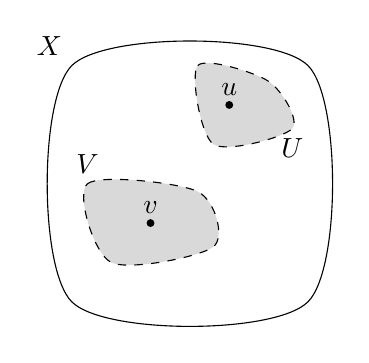
\begin{tikzpicture}
		\draw plot[smooth cycle] coordinates{(0,0) (3,0) (3,3) (0,3)};
		\draw (0,3) node[anchor=south east]{$ X $};

		\filldraw[dashed, fill = gray!30] plot[smooth cycle] coordinates{(1.8,2) (1.6,3) (2.5,2.8)
			(2.8,2.2)};
		\draw (2.8,2.2) node[below]{$ U $};
		\fill (2,2.5) circle (0.05) node[above]{$ u $};

		\filldraw[dashed, fill = gray!30] plot[smooth cycle] coordinates{(0.5, 0.5)
			(0.2, 1.5) (1.6,1.4) (1.8, 0.7)};
		\draw (0.2, 1.5) node[above]{$ V $};
		\fill (1,1) circle (0.05) node[above]{$ v $ };
	\end{tikzpicture}
\end{document}
